%%%%%%%%%%%%%%%%%%%%%%%%%%%%%%%%%%%%%%%%%%%%%%%%%%%%%%%%%%%%%%%%%%%%
%% I, the copyright holder of this work, release this work into the
%% public domain. This applies worldwide. In some countries this may
%% not be legally possible; if so: I grant anyone the right to use
%% this work for any purpose, without any conditions, unless such
%% conditions are required by law.
%%%%%%%%%%%%%%%%%%%%%%%%%%%%%%%%%%%%%%%%%%%%%%%%%%%%%%%%%%%%%%%%%%%%

\documentclass[
  digital, %% This option enables the default options for the
           %% digital version of a document. Replace with `printed`
           %% to enable the default options for the printed version
           %% of a document.
  table,   %% Causes the coloring of tables. Replace with `notable`
           %% to restore plain tables.
  lof,     %% Prints the List of Figures. Replace with `nolof` to
           %% hide the List of Figures.
  lot,     %% Prints the List of Tables. Replace with `nolot` to
           %% hide the List of Tables.
  %% More options are listed in the user guide at
  %% <http://mirrors.ctan.org/macros/latex/contrib/fithesis/guide/mu/sci.pdf>.
]{fithesis3}
%% The following section sets up the locales used in the thesis.
\usepackage[resetfonts]{cmap} %% We need to load the T2A font encoding
\usepackage[T1,T2A]{fontenc}  %% to use the Cyrillic fonts with Russian texts.
\usepackage[
  main=english,  %% By using `czech` or `english` as the main locale
                %% instead of `slovak`, you can typeset the thesis
                %% in either Czech or English, respectively.
  english, german, russian, czech, slovak %% The additional keys allow
]{babel}        %% foreign texts to be typeset as follows:
%%
%%   \begin{otherlanguage}{german}  ... \end{otherlanguage}
%%   \begin{otherlanguage}{russian} ... \end{otherlanguage}
%%   \begin{otherlanguage}{czech}   ... \end{otherlanguage}
%%   \begin{otherlanguage}{slovak}  ... \end{otherlanguage}
%%
%% For non-Latin scripts, it may be necessary to load additional
%% fonts:
\usepackage{paratype}
\def\textrussian#1{{\usefont{T2A}{PTSerif-TLF}{m}{rm}#1}}
%%
%% The following section sets up the metadata of the thesis.
\thesissetup{
    date            = \the\year/\the\month/\the\day,
    university      = mu,
    faculty         = sci,
    department      = Ústav chemie,
    departmentEn    = Department of Chemistry,
    extra = {
      departmentCs  = Department of Chemistry,
    },
    programme       = Fyzikální chemie,
    programmeEn     = Physical Chemistry,
    extra = {
      programmeCs   = Chemistry,
    },
    field           = Fyzikální chemie,
    fieldEn         = Physical Chemistry,
    extra = {
      fieldCs       = Physical Chemistry,
    },
    type            = mgr,
    author          = Petra Hrozková,
    gender          = f,
    advisor         = doc. Markéta Munzarová Dr. rer. nat. ,
    title           = Studium elektronové struktury fosfosilikátů a jejich silikátových          prekurzorů metodou DFT,
    TeXtitle        = A DFT study of the Electronic Structure of Silicate Precursors for Phosphosilicates
.
,
    titleEn         = A DFT study of the Electronic Structure of Silicate Precursors for Phosphosilicates
,
    TeXtitleEn      = A DFT study of the Electronic Structure of Silicate Precursors for Phosphosilicates
,
    extra = {
      titleCs       =A DFT study of the Electronic Structure of Silicate Precursors for Phosphosilicates
,
      TeXtitleCs    = A DFT study of the Electronic Structure of Silicate Precursors for Phosphosilicates
,
    },
    keywords        = {kľúčové slovo 1, kľúčové slovo 2, ...},
    TeXkeywords     = {kľúčové slovo 1, kľúčové slovo 2, \ldots},
    keywordsEn      = {keyword1, keyword2, ...},
    TeXkeywordsEn   = {keyword1, keyword2, \ldots},
    extra = {
      keywordsCs    = {klíčové slovo 1, klíčové slovo 2, ...},
      TeXkeywordsCs = {klíčové slovo 1, klíčové slovo 2, \ldots},
    },
    abstract      = {This is the abstract of my thesis, which can

                     span multiple paragraphs.},
    abstractEn    = {This is the English abstract of my thesis, which can

                     span multiple paragraphs.},
    extra = {
      abstractCs   = {This is the Czech abstract of my thesis, which can

                      span multiple paragraphs.},
    },
    thanks        = {These are the acknowledgements for my thesis, which can

                     span multiple paragraphs.},
    bib           = example.bib,
    %% Uncomment the following line (by removing the % symbol at
    %% the beginning) and replace `assignment.pdf` with the
    %% filename of your scanned thesis assignment.
    % assignment    = assignment.pdf,
}
\usepackage{makeidx}      %% The `makeidx` package contains
\makeindex                %% helper commands for index typesetting.
%% These additional packages are used within the document:
\usepackage{paralist} %% Compact list environments
\usepackage{amsmath}  %% Mathematics
\usepackage{amsthm}
\usepackage{amsfonts}
\usepackage{url}      %% Hyperlinks
\usepackage{mhchem}
\usepackage{subfigure}
\usepackage{listings} %% Source code highlighting
%\usepackage{chemmacros}

\lstset{
  basicstyle      = \ttfamily,%
  identifierstyle = \color{black},%
  keywordstyle    = \color{blue},%
  keywordstyle    = {[2]\color{cyan}},%
  keywordstyle    = {[3]\color{olive}},%
  stringstyle     = \color{teal},%
  commentstyle    = \itshape\color{magenta}}
\usepackage{floatrow} %% Putting captions above tables
\floatsetup[table]{capposition=top}
\begin{document}




\chapter{Teoretický úvod}

\section{Experimentální podklady}
Cílem práce je podat vysvětlení některých experimentálních jevů, které byly pozorovány u silikofosfátových polymerů. Těmto sloučeninám se již dříve věnovala pozornost kolegů z materiálové chemie. Silicofosfátové polymery mají potenciál jako porézní materiály, které obsahují opakující se skupiny Si-O-P\cite{Styskalik2015thesis}.
Naše pozornost se zameřila na přítomnost hypervalentního křemíku, fosfátových a karbonylových esterů v těchto polymerech. Modely, které měly reprezentovat vybrané části z těchto polymerů, se dělily na dvě části. První část tvořily skutečně pozorované struktury a druhou část tvořily teoretické struktury, kde byly vybrané fosfátové skupiny nahrazeny karbonylem. Důležitým srovnávacím parametrem mezi toeretickými modely a experimentem se stala spektroskopická data, konkrétně NMR parametry.

\subsection{Silikofosfátové polymery}
 V přírodě se křemík ve svých sloučeninách vyskytuje běžně jako čtyřvazný s přímou vazbou na kyslík a to především ve formě křemičitanů. Zajímavostí je minerál thaumasit, kde se křemík vyskytuje jako \ce{SiO6}. Zjednodušená struktura připravených silikofosfátu je na obrázku \ref{si_polymer_cely}. Ve strukturách byly identifikovány tři druhy koordinačního okolí křemíku. Jeden tetraedricky koordinovaný křemík a dva oktaedricky koordinované křemíky. Silikofosfáty jsou homogenní a amorfní sloučeniny a proto je obtížné určit přesnou strukturu \cite{Styskalik2015thesis}. Důležitou vlastnotstí silikofosfátů je schopnost tvořit vnitřní cykly pomocí skupiny Si-O-P různých velikostí a vytvážet porézní struktury. Ve strukturách byl pozorován jev, že když je kyslík nahrazen uhlíkem přímou vazbou na křemík, tak je ovlivněna nejen velikost cyklů, ale i schopnost jeho koordinace.
\begin{figure}[h!]
\caption{Silikofosfátová síť, \cite{Styskalik2015thesis}. }
  \center
  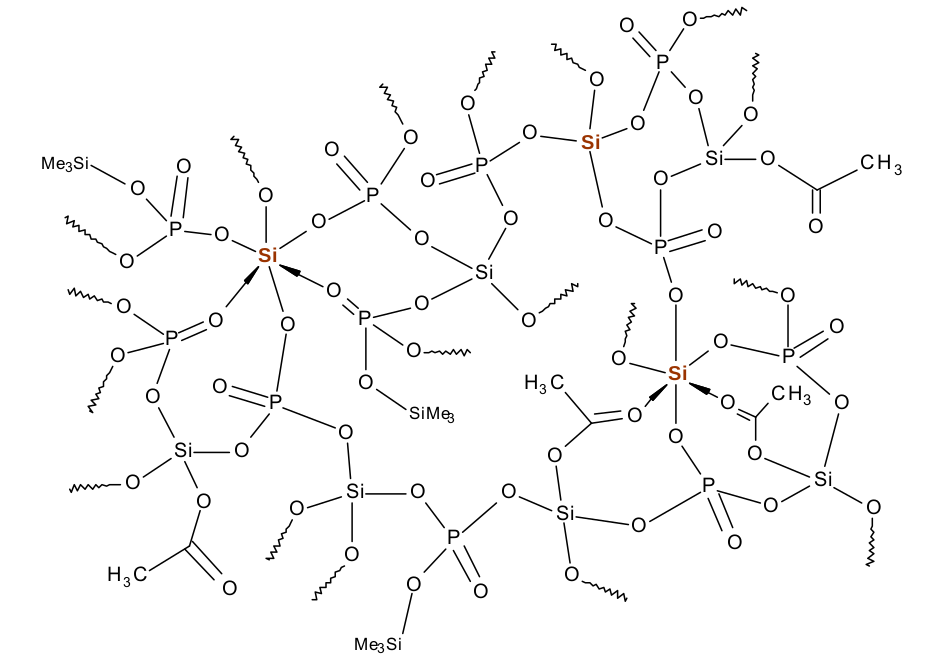
\includegraphics[width=12cm]{si_polymer_cely.png}
  \label{si_polymer_cely}
  \end{figure}
  Konkrétní metody příprav slikofosfátových sloučenin jsou uvedeny například v práci Mgr. Aleše Stýskalíka, PhD  \cite{Styskalik2015thesis}.

\subsubsection{Křemík jako hypervalentní sloučenina}
Sloučeniny, kde se vyskytuje jeden nebo více atomů s více než osmi elektrony (oktet) se nazývají hypervalentní/hyperkoordinované. Sloučeniny zároveň musí být schopné vytvořit více vazeb než je číslo jejich atomových orbitalů. V případě prvků p-skupiny to znamená, že jsou schopny tvořit více než čtyři vazby, obvykle počet vazeb je pět nebo šest. Konkrétně křemík může vytvářet 4-,5- a 6- koordinované sloučeniny a stát se hypervalentní. Silikofosfáty vznikají substitucí křemíku za P-OH skupiny. Díky podobnosti křemíku a fosforu jsou tyto dva atomy ve svých sloučeninách snadno zaměnitelné. \\

První hypervalentní sloučeniny křemíku byly připraveny už v devatenáctém století. Jako ligand musely být použity vysoce elektronegativní prvky, tento jev však byl objasněn až mnohem později. V prvních sloučeninách byl elektronegativním ligandem fluor, \ce{(SiF6)^{2-}} a \ce{(Si(NH2)2F3)^{2-}}. Nejvýznamější objevy v oblasti hypervalentních struktur byly ale uskutečněny až v nedávné době a to především díky pokročilejším zobrazovacím analytickým metodám. Podrobnější pohled na hypervalentní struktury křemíku, vazebné poměry a možnosti přípravy jsou shrnuty například v literatuře \cite{Wagler2014}.\\

\subsubsection{Fyzikální a chemické vlastnosti silikofosfátových sloučenin}
Samotné silikofosfátové polymery mají zajímavé fyzikální a chemické vlastnosti. Příkladem je Brønstedovská kyselost nebo vysoká protonová vodivost. Jedno z možných uplatnění silikofosfátových polymerů mohou být konduktory, elektrolyty, optická vlákna a biokompatibilní materiály. Fyzikální a chemické vlastnosti lze dobře vysvětlit pomocí analýzy molekulových orbitalů. Obecně mají Lewisovské kyseliny prázdné molekulové orbitaly, které leži dostatečně blízko obsazeným MO \footnote{MO = Molekulový orbital} konjugované báze. Vazba mezi křemíkem a jeho ligandem je silně ovlivněna elektronegativitou donorního ligandu. Atomy jako uhlík, dusík, kyslík, fluor nebo chlor podporují navyšování koordinace křemíku. V případě čtyřkoordinovaných sloučenin křemík poskytuje do vazeb všechny své valenční elektorny. Ve vyšším koordinačním stupeni už může křemík poskytnou pouze prázdné orbitaly a proto chová se jako Lewisovská kyselina.\\

Vazbu mezi křemíkem a kyslíkem lze považovat za dobrou Lewisovskou kyselinu. Z experimentu je známo, že \ce{SiO4} je dostatečnou Lewisovskou kyselinou, aby křemík mohl přímo reagovat s Lewivoskou bazí. Pokud je jeden z kyslíku ve struktuře nahrazen uhlíkem, schopnost navyšovat koordinaci je ztracena. Stejný jev pozoroval Aleš Sýskalík a spol. \cite{Styskalik2015thesis} a to vedlo k hypotéze o snížení Lewisovské kyselosti křemíku při tvorbě přímé vazby Si - C. Naopak pětikoordinovaný křemík je lepší Lewisovskou kyselinou než čtyřkoordinovaný a hypervalency podporuje.\cite{Wagler2014}\\

\begin{figure}[h!]
\caption{\cite{hypervalentsiliconmacmillangroup2005}}
  \center
  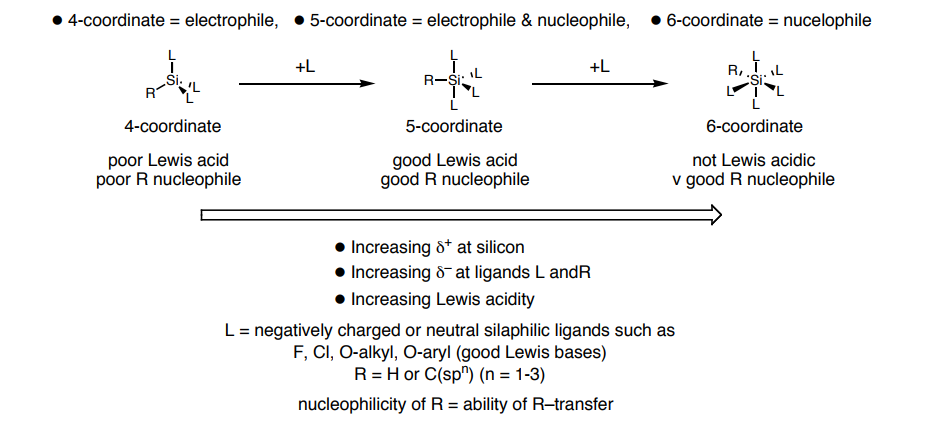
\includegraphics[width=12cm]{schema_silicophosphates.png}
  \label{schema_silicon_coordinate}
  \end{figure}

Pro vysvětlení hypervalence křemíku lze použít teorii hybridizace. Obecně se čtykoordinované sloučeniny vyskytují jako tetraedry, hybridizace $sp^3$. Pětikoordinované sloučeniny tvoří trigonální bipyramidu, hybridizace $sp^3d$. A šestikoordinované sloučeniny tvoří oktaedr, hybridizace $sp^3d^2$. (obrázek?) \\

Čtyřkoordinovaný křemík slňuje tetraedrické uspořádání. Při zvýšení koordinace na pět by měla být pozorována trigonální bipyramida, $sp^3d$. Výskyt $d$ orbitalu ve vazbě ale způsobuje nárust energie vazby na více než 200 kcal/mol. Z tohoto důvodu se předpokládá, že $d$ orbitaly se podílejí pouze na polarizaci porbitalů. Pentavalentní koordinace je poté realizována jako $3sp^2$ hybridizace doplněna třícenterní, čtyřelektronovou vazbou $3c-4e$ s p orbitalem.
 V případě pětikoordinované sloučeniny se ale spíše uvažuje hybridizace $sp^2$ a jedna vazba $3c-4e$ s p orbitalem, právě kvůli energii $d$ orbitalů. (obrázek?) \\
 Hypervalentní sloučeniny jsou lepší Lewisovské kyseliny díky d+ efektu na centralním křemíku. Důvodem je přesun elektronové hustoty na ligandy skrz nevazebné MO a podpora $3c-4e$ vazby. Rozložení elektronové hustoty molekulu stabilizuje a z tohoto důvodu se v hypervalentních sloučeninách vyskytují jako ligandy prvky s vysokou elektronegativitou. Tento jev dobře popisuje tzv. Benovo pravidlo:"Elektronegativní prvek dáva přednost vazbe s větším p-charakterem."\cite{hypervalentsiliconmacmillangroup2005}.\\
Pro křemík v koordinaci šest lze také předpokládat, že význam $d$ orbitalů nebude významný vzhledem k jejich energii. I zde se do vazby zapojí $3c-4e$ vazby\cite{Wagler2014}.\\

Další možnost interpretace hypervalence je založena na vysoké iontovosti vazby na křemíku. Obecně iontovost s koordinačním číslem roste.
Navíc chování vazby Si-ligand silně závisí na samotném ligandu a sterickém a elektronovém uspořádání. Hovoříme o Lewisovské kyselosti křemíkové vazby s elektronegativním atomem. Chování křemíku lze rozdělit na iontové, sigma vazebné a donor interakci.\cite{Wagler2014}\\

Z tohoto důvod jsme se rozhodli porovnávat Lewivoskou kyselost, abychom určili stabilitu jednotlivých částí silikofosfátů. Navíc jsme se snažili najít parametr, který by umožnil určit velikost póru v závislosti na okolí křemíku. Jako prostředek ke zkoumání silikofosfátů jsem zvolila molekulové orbitaly, které poskytují široké spektrum informací o molekule, vazbách, struktuře, kyselosti,..  Analýza byla provedena s pomocí teorie funkcionální hustoty(DFT)\footnote{DFT - Density Functional Theory, česky Teorie funkcionálu hustoty}, která se řadí mezi kvatově-chemické metody. Pro porovnání byla stejná analýza udělána s pomocí teorie Přirozených molekulových orbitalů(NBO)\footnote{NBO - Natural Bond Orbitals, česky Přirozené Molekulové orbitaly}. Výhoda přístupu NBO je snadnější převod čísel do chemického významu.


\section{Metody kvantové chemie}
Chemické vlastnosti molekul jsou určeny elektrony. Elektrony se řadí mezi elementární částice a proto pro jejich popis nelze použít běžnou newtonovskou mechaniku. Chování elektronů popisuje Schrödingerova rovnice, která se řadí mezi diferenciální rovnice druhého řádu. Její exatní řešení existuje pouze pro velice malé systémy, konkrétně systémy s dvěma částicemi. Z tohoto důvodu je v chemických aplikavích nutno použít zjednodušení. Základem je Born-Oppenhemrova aproximace(B-O) \ref{B_O_approximace}, která předpokládá, že pohyb elektronů a jader lze oddělit a Vlnová funkce elektronů závisí pouze na poloze jader, ne jejich rychlosti. Vlnová funkce se rozpadá na dvě části, elektronovou a jadernou. Řešení se redukuje na 3N prostorových souřadnic. Zároveň je vlnová funkce parametricky závislá na poloze jader, pro každou geometrii jader je získána jiná vlnová funkce. Ve druhém kroku dostaneme plochu potenciální energie (PES)*/footnote{PES - Potential Energy Surface} pro každou geometrii a Schodingerova rovnice najednou závisí pouze na 3N prostorových souřadnících elektornů \cite{lechamolecularmodeling}.

 Dalšík krokem je Hartree-Fockova metoda (HF), někdy nazývána self-konzistentní metoda. HF využívá principů z Hartreeho metody, kdy se elektron pohybuje v časově průměrném poli ostatních elektronů, vlnová funkce je součin jednoelektronových funkcí. Výsledná vlvnová funkce je nalezena s pomocí variačního principu jako ta s nejnižší enenrgií. Orbitaly musí ortogonální a ortonormální.
 \begin{equation}
 S_{ii} = \int \psi_i * \psi_i dx dy dz = 1 ~ \wedge ~ S_{ij} = \int \psi_i * \psi_j dx dy dz = 0
 \end{equation}

\begin{equation}
  \Psi_{total} = \Psi_{electronic} \cdot \Psi_{nuclear}
  \label{B_O_approximace}
\end{equation}
Výsledkem je energie a uspořádání elektronů pro každou vzájemnou polohu jader.
\begin{equation}
\Psi_{total} = \Psi_{electronic} \cdot \Psi_{nuclear}
\end{equation}
Původní Hartreeho metoda neobsahovala antisymetrii. Tu později doplnil Vladimir Aleksandrovič Fock a John Slater. Výsledke je Hartree-Fockova metoda self-konzistentního pole(HF-SCF). Nejnižěí energie se hledá pomocí variačního počtu. Vlnovou funkci lze zapsat jako Slaterův determinant, který zaručuje antisymetrii vlnové funkce vůči výměně polohových a spinových souřadnic \ref{Slateruv_determinant}.
\begin{equation}
\psi =  \frac{1}{\sqrt{N!}}\begin{vmatrix}
\psi_1(1)\alpha(1) & \psi_1(1) \beta (1)  & \dots & \psi_{n/2}(1)\beta(1) \\
\psi_1(2)\alpha(2) & \psi_1(2) \beta (2) & \dots & \psi_{n/2}(2)\beta(2) \\
\vdots             & \vdots                           & \ddots & \vdots \\
\psi_1(n)\alpha(n) & \psi_1(n) \beta (n) & \dots & \psi_{n/2}(n)\beta(n)
\end{vmatrix}
\label{Slateruv_determinant}
\end{equation}
$\psi_i$ je jednoelektronová vlnová funkce, $s_j$ jsou elektrony, $\sqrt{N!}$ je normalizační faktor.
 Nevýhoda HF-SCF přístupu je fakt, že neuvažuje korelaci elektronového pohybu. Tento jev v sobě zahrnují metody, které jsou rozšířením HF, jako například poruchova teorie (MBPT)*/footnote{MBPT - Many-Body Pertrubation theory}, metoda konfigurakční interakce (CI)*/footnote{Configuration Interaction} nebo clustrové metody (CC)*/footnote{Coupled
Cluster methods}. Časová složitost těchto metod je uvedena na obrázku. Velkou výhodou těchto metod je jejich přesnost, bohužel vzhledem k časové náročnosti je lze použít pouze pro malé systémy.

\subsection{Bázové funkce}
Data z experimentu mohou pomoci s výběrem vhodné výpočetní metody. Jedním z přístupů je model bázových funkcí, kdy jsou MO hledány jako kombinace sady bázových funkcí. Podle postulátu QM o úplných vlastních hodnotách uplných Hermitovských operátorů lze každý molekulový orbital sestrojit jako lineární kombinaci atomových orbitalů, tzv. LCAO*/footnote{LCAO - Linear Combination of Atomic Orbitals.}. Konkrétně jsou AO sestaveny jako kombinace orbitalů Gaussovského (GTO) nebo Slaterova typu(STO).
Kompletní sada bázovýchh funkcí obsahuje nekonečně mnoho funkcí, což dělá problém neřešitelný. Vhodný konečný počet funkcí byl určen s pomocí ladění chyb a poskytuje dostatečně přesné výsledky za příměřenou cenu. Každá elektronové korelačních metod škáluje rozdílně podle počtu elektronů(určeno počty obsazených MO) a podle sady bázových funkcí (počet neobsazených, virtuálních, MO).\\
Minimální sada bázových funkcí v sobě obsahuje elektrony v základním stavu. Naopak rozšířená sada bázových funkcí v sobě obsahuje polorizační funkce nebo difúzní funkce. Typ bázových funkcí mohou být vodíkového typu, GTO nebo STO. Nevýhoda funkcí vodíkového typu je délka výpočtu. STO oproti tomu nemají žádné radiální uzly a jejich sčítání není lineární. Vhodnou aproximací jsou orbitaly gaussovského typu, které sice nemají vhodné chování na jádře, ale platí pro ně pravidlo, že součet GTO je opět GTO.\cite{lowe2011quantum}

Sada bázových funkcí přirozených atomových orbitalů je příkladem zmenšením báze. Přirozené orbitaly jsou takové, které diagonalizují matici hustoty a počet elektronů v orbitalu odpovídá obsazovacímu čísli.

\subsubsection{Effective Core Potential Basis Sets (ECP)}
Systém s velkým počtem core, vnitřních, elektronů, jsou časové náročné. Často to jsou prvky za třetí periodou. Z pohledu chemické vazby je možno vliv core elektronů považovat za méně důležitý. Stejná situace nastává ve chvíli, kdy je v systému příliš mnoho elektornů. Jednoduše, systém je příliš velký. V obou případech lze použít funkci, ktra bude modelovat chování core elektronů. ECP má čtyři hlavní kroky. Prvním krokem je, že vlnová funkce pro všechny elektrony je vytvořdna s pomocí HF metody. Valenční orbitaly jsou nahrazeny skupinou psudoorbitalů bez nodálních ploch.

\section{Density functional theory (DFT)}
Elektronová struktura každého chemického systému je popsána jako mnohoelektornová funkce. Tři možnosti korelace pohybu elektronů jsou popsány v kapitole ... . Tady bych ráda zmínila, že tradiční ab inito metody zahrnující elektronové korelace mají dvě nevýhody, výpočetní náročnost a složitost.

Teorie funkcionálu hustoty\footnote{Z matematické analýzy je funkcionál operátor zobrazení z množiny funkcí do množiny obecně komplexních čísel.}poskytuje řešení pro velké systémy. Myšlenka DFT dává pohled na elektronovou strukturu z úplně jiného úhlu. DFT je kvantově mechanické modelování používané v chemii, fyzice a materiálových vědách. Existuje spojitost mezi elektronovou hustotou systému a jeho energií.
Výhodou DFT přístupu je fakt, že funkcí pouze tři souřadnic, nezávislé na počtu elektronů a počet proměnných je nezávislý na velikosti systému. Jeden z výsledků DFT je korelace energie. Energie je určena jako funkce elektronové hustoty. Přesný funkcionál mezi energii a elektronovou hustotou není doposud znám. Funkcionály lze rozdělit do tří částí, stejně jako vlnovou funkci. Kinetická energie, přitahování elektronů a jader a repulze mezi elektrony(E-E). Elektronová repulze se skládá z Columbovské části a Výměnné části. Tento model je aproximací pro elektronový plyn, z tohoto důvodu je pro chemii nepoužitelný. Na druhou stranu je to dobrý model, kde lze začít.


Nevýhoda modelu bez interakcí je celková chyba, která dosahuje 15-50\%. V tomto modelu nelze mluvit o existenci molekul.\cite{jensen2007introduction}

Moderní DFT metody se začaly objevovat po roce 1964 jako výsled dvou teorému. Trvalo to bezmála 40 let od modelu elektronového plynu. Prvním je Hohenberg-Kohn teorém (H-K), který mluví o základním stavu. Vnější potenciál  $V_ext$ je jednoznačnná funkce elektronové hustoty $\varrho$. Všechny vlasnosti základního stavu mnohaelektronového systému jsou určeny elektronovou hustotou. Nevýhodou je, že elektronovou hustotou je určen pouze základní stav a pro excitované stavy jej nelze použít.

Samotná elektronová hustota je výsledkem druhého teorému. Ten říká, že nalezená elektornová hustota je jediná správná. Využívá variačního principu pro určení elektronové hustoty bez vlnové funkce. Správná elektronová hustota musí mít nejnižší energii a nejpřesnější energii. Energie excitovaného stavu musí být nižší než energie elektroové hustoty ostatních elektronů. Pro výpočetní chemii mají větší význam Kohn-Shamovy orbitaly. Kinetická energie se rozpadá na dvě části. Exaktní a korekční část. \cite{jensen2007introduction}\cite{koch2000chemist}
Slaterův determinant odpovídá interakci elektronů. Přesná kinetická energie je spojená s přirozenými orbitaly. Funkcionál pro nejmenší energii představuje základní stav mnohaelektronvého systému.

\begin{equation}
  E[\varrho] = \int \varrho(r)v(r)dr + F[\varrho] \quad F[\varrho] = T[\varrho] + V_{ee}[\varrho]
\end{equation}
Tomas-Fermi model ztrácí přesnost, protože uvažuje eletronovou hustotu samostatně. K-S ke kinetické energii  $T[\varrho]$ přistupuje nepřímo a umožňuje použít DFT pro praktické použití při výpočtech. \cite{parr1994density}

\section{Přirozené orbitaly (NBO)}
Přirozené molekulové orbitaly \footnote{NBO - Natural Bond orbital} jsopou odlišným pohledem na chemickou vazbu. Existuje spoustu přístupů k analýze vlnové funkce. Schrödingerova rovnice určuje energii pro každou vlnovou funkci. Vlnová funkce určuje pozici elektronů i jader. Jak je možné určite, zda jsou dva atomy spojené vazbou? Dobrým příkladem parametru, který lze použít pro určení vlasnosti molekul je atomový náboj. Obvyklé metody pro přiřazení náboje elektronu je analýza založená na bázových funkcí, elektrostatické potenciálu nebo vlnové funkci, lokalizovaných orbitalech nebo přirozených orbitalech. \\
První přístup používá MO a matici hustoty (DS)\footnote{DS - Density Matrix} a Mullikenovu populační analýzu. Čiste matematikcým přístupem je těžké určit správný výsledek. Sada populačních nábojů neodpovídá skutečným multipole moment.

Lepší přístup pro popis náboje je elektrostatický potenciál. Náboj je silně spojen s force field method. Nevazebné interakce josu popsány jako část elektrostatické interakce. Cčsitě matemtický přístup poskytuje metoda AIM\footnote{AIM = Atoms in Molecules}. Elektronová hustota může být vyhodnocena jako normální funkce, která má své minimum, maximum nebo sedlové body. Hranice mezi dvěma atomy v tři dimenzionálním prostoru prostorem s dvěmi dimenzemi. \\
Dalším způsobem vyhodnocení jsou Lokalizované Orbitaly (NO).  První řád matice je diagonalizován a jeho vlastní vektory jsou označeny jako přirozené orbitaly. Vlastní hodnoty jsou obsazovací čísla. NO dávájí nejrychlejší konvergenci a mohou popsat rozložení elektronů v atomech a odvození atomového náboje a vazby.  \cite{jensen2007introduction} \\
 NO jsou teoretickým zjednodušením, které určuje elektronovou hustoty v atomech a  tento přístup odpovídá přístupu Lewisovských struktur. NO byly objeveny v roce 1955 Per-Olov Lödwin. NO mohou být vyvořeny z Slaterova determinantu. K-S nemají fyzikální význam a je zde problém s interpretací výsledků. Ale platí, že HF i K-S orbitaly mohou být použity pro tvorbu sady přirozených vazebných orbitalů. Přiozené orbitaly jsou vytvořeny diagonalizací matice hustoty
(NBO program)

Lepší sada orbitalů se nazývá "přirozené" a jsou schopné zahrnout korelaci $\varrho$(r). Přirozené orbitaly mají maximální ovsazenost a jsou určené ze samotné vlnové funkce.

\section{Tvrdost a měkkost kyselin a báze}
Chemickí tvrdost a měkkost má pro experimentální chemii velký význam . S pomocí analýzy tvrdosti/měkkost může být predikován produkt reakce a jeho stabilita. Bylo pozorováno, že reakce dvou tvrdých molekul poskytuje stabilní produkt, stejně to platí i pro reakci dvou měkkých molekul. \\
Globální tvrdost a měkkost můžou být použity pro celou molekulu. Jednotlivé atomy mají tvrdost a měkkost lokální. Tuto vlastnost lze interpretovat jako lokální náboj. Globální vlastnosti pochází z energie HOMO a LUMO orbitalů. Určení lokálních vlastností je obtížné, protože jsou spojeny s Fukuiho rovnicí. Ty popisují, který atom v molekule přijme nebo ztratí elektron. Chemická interpretace je schopnost nuklefilního nebo elektrofilního útoku. Stejně dobře to popíše externí elektrické pole a polarizace. Toto je přímo spojené s elektronovou hustotou a DFT metodami.

Elektrofilita atomu A v molekule M s N elektrony.
\begin{equation}
f_A^+ = P_A(N+1) - P_A(N)
\end{equation}
Nuklefilita atomu A v molekule M s N elektrony.
\begin{equation}
f_A^- = P-A(N) - P_A(N-1)
\end{equation}
Radical attack susceptibility of atom A in molecule M with N electrons.
\begin{equation}
f_A^0 = \frac{1}{2}[P_(N+1) - P_A(N-1)]
\end{equation}

Nalezení obsazovacího čísla na každém atommu je citlivé na výběru baze. Příliš velká baze dává špatné výsledky.


\section{Výpočetní část}
Výpočetní část byla rozdělena do tří částí. První část se zabývá stukturami, druhá část dává podrobnější pohled na vazby ve zvolených strukturách a třetí, poslední, část se zaměřuje na spektroskopii.
Cílem strukturní bylo modelovat části struktur silikofosfátů metodami DFT. Struktura silikofosfátu byla rozdělena do tři skupin, aby co nejlépe popsala jevy, které se tam objevují. Vazby byly analyzovány metodou NBO a analýzou složení kanonických orbitalů. Poslední část, která se věnuje spektroskopii, dává pohled na NMR parametry.

\subsection{Struktury}
Struktury pro teoretickou část jsou rozděleny podle velikosti a zároveň podle stupně koordinace křemíku.
\subsubsection{Malé modely}

\subsubsection{Středně velké modely}
Tato část se věňuje nejmenším možným modelům, které již tvoří uvnitř svých struktur cyklus. Jako referenční molekula byl použita \ce{(acetylmethoxyl)trifluorsilan} z článku \ref{Chipanina2011}. Strutktura \ce{(acetylmethoxyl)trifluorsilan} slouží jako model křemíku v koordinaci čtyři, který má ve svém okolí vysoce elektronegativní atomy. To podporuje teoretické předpoklady o hypervalenci křemíku, pokud má ve svém okolí silně elektronegativní prvek.
\begin{figure}
\begin{center}
\subfigure[(acetylmethoxyl)trifluorsilan]{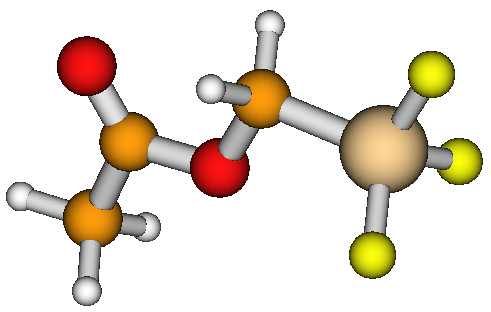
\includegraphics[width=5cm]{acetylmethyltrifluor.png} \label{obr_h4sio4_MO_s1_1}}
\subfigure[]{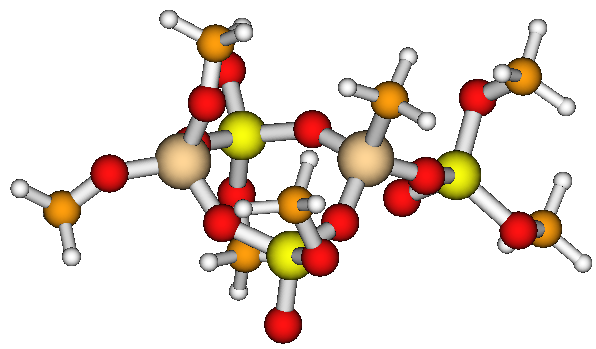
\includegraphics[width=5cm]{si_model_methyl.png}\label{obr_h4sio4_MO_s1_20}}
\subfigure[]{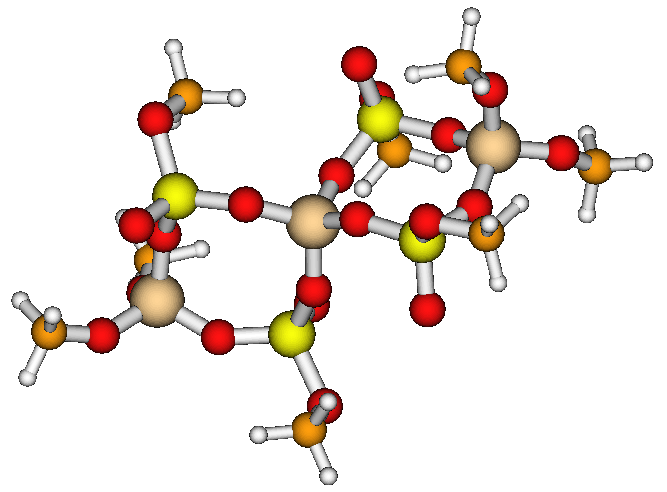
\includegraphics[width=5cm]{si_model_orezany.png}\label{obr_h4sio4_MO_s1_24}}
\caption{}

\label{obr_h4sio4_vysledky_I}



\end{center}
\end{figure}
Pro zvolené sloučeniny byla provedena analýza kanonických orbitalů, výsledky jsou uvedeny v tabulce.
\subsubsection{Velké modely}




\subsection{Vazby}

\subsection{Spektroskopi}














{\csname captions\languagename\endcsname %% Temporarily override
%% the BibLaTeX localization with the original babel definitions.
\makeatletter %% Use the correct localization of the quotations.
  \thesis@selectLocale{\thesis@locale}\makeatother
\printbibliography[heading=bibintoc]} %% Print the bibliography.
\appendix %% Start the appendices.




\end{document}
